\pdfminorversion=4
\documentclass[aspectratio=169]{beamer}

\mode<presentation>
{
  \usetheme{default}
  \usecolortheme{default}
  \usefonttheme{default}
  \setbeamertemplate{navigation symbols}{}
  \setbeamertemplate{caption}[numbered]
  \setbeamertemplate{footline}[frame number]  % or "page number"
  \setbeamercolor{frametitle}{fg=white}
  \setbeamercolor{footline}{fg=black}
} 

\usepackage[english]{babel}
\usepackage[utf8x]{inputenc}
\usepackage{tikz}
\usepackage{courier}
\usepackage{array}
\usepackage{bold-extra}
\usepackage{minted}
\usepackage[thicklines]{cancel}
\usepackage{fancyvrb}

\xdefinecolor{dianablue}{rgb}{0.18,0.24,0.31}
\xdefinecolor{darkblue}{rgb}{0.1,0.1,0.7}
\xdefinecolor{darkgreen}{rgb}{0,0.5,0}
\xdefinecolor{darkgrey}{rgb}{0.35,0.35,0.35}
\xdefinecolor{darkorange}{rgb}{0.8,0.5,0}
\xdefinecolor{darkred}{rgb}{0.7,0,0}
\definecolor{darkgreen}{rgb}{0,0.6,0}
\definecolor{mauve}{rgb}{0.58,0,0.82}

\title[2019-10-17-pyhep-awkward]{Uproot and Awkward-Array in the Year of Python}
\author{Jim Pivarski}
\institute{Princeton University -- IRIS-HEP}
\date{October 17, 2019}

\usetikzlibrary{shapes.callouts}

\begin{document}

\logo{\pgfputat{\pgfxy(0.11, 7.4)}{\pgfbox[right,base]{\tikz{\filldraw[fill=dianablue, draw=none] (0 cm, 0 cm) rectangle (50 cm, 1 cm);}\mbox{\hspace{-8 cm}
\includegraphics[height=1 cm]{princeton-logo-long.png}\hspace{0.1 cm}\raisebox{0.1 cm}{
\includegraphics[height=0.8 cm]{iris-hep-logo-long.png}}\hspace{0.1 cm}}}}}

\begin{frame}
  \titlepage
\end{frame}

\logo{\pgfputat{\pgfxy(0.11, 7.4)}{\pgfbox[right,base]{\tikz{\filldraw[fill=dianablue, draw=none] (0 cm, 0 cm) rectangle (50 cm, 1 cm);}\mbox{\hspace{-8 cm}
\includegraphics[height=1 cm]{princeton-logo.png}\hspace{0.1 cm}\raisebox{0.1 cm}{
\includegraphics[height=0.8 cm]{iris-hep-logo.png}}\hspace{0.1 cm}}}}}

% Uncomment these lines for an automatically generated outline.
%\begin{frame}{Outline}
%  \tableofcontents
%\end{frame}

% START START START START START START START START START START START START START

\begin{frame}{}
\huge
\vspace{1 cm}
\begin{center}
\textcolor{darkblue}{Year of Python?}
\end{center}
\end{frame}

\begin{frame}{On Scientific Linux, uproot/awkward is installed as often as Pandas}
\vspace{0.5 cm}
\begin{columns}
\column{1.2\linewidth}
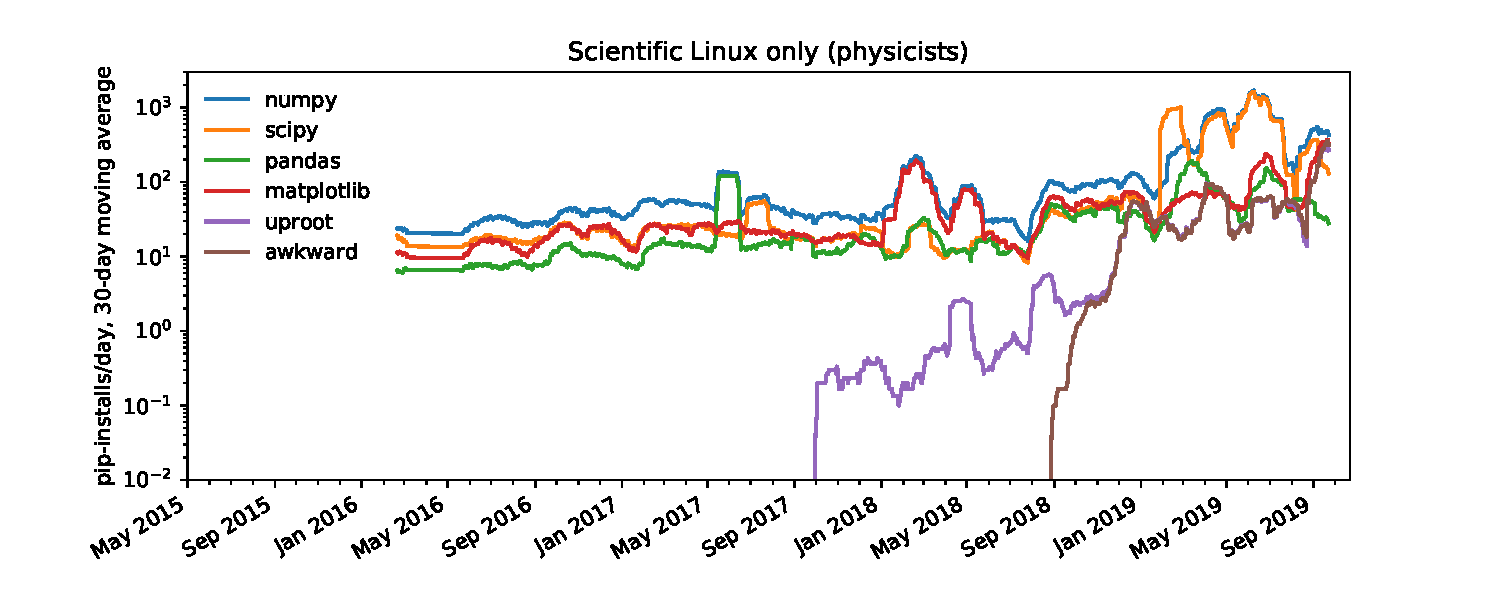
\includegraphics[width=\linewidth]{pip-scilinux-uproot.pdf}
\end{columns}
\end{frame}

\begin{frame}{And so is Coffea\ldots}
\vspace{0.5 cm}
\begin{columns}
\column{1.2\linewidth}
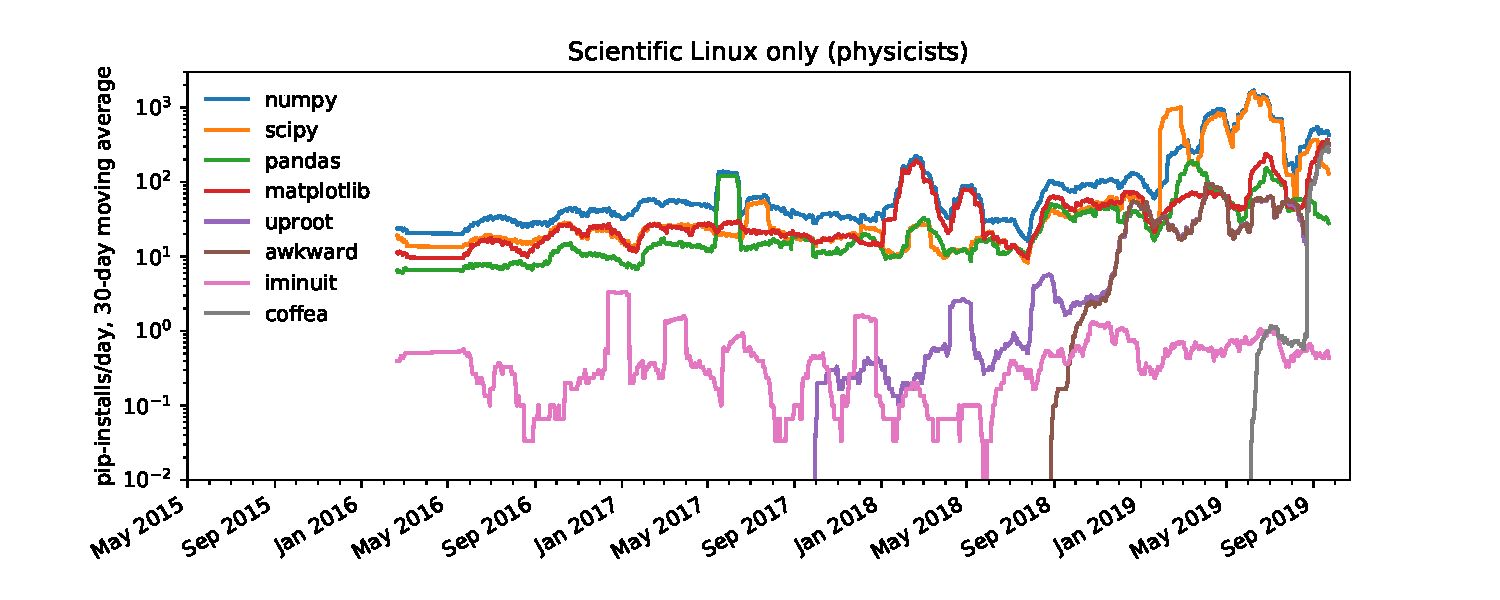
\includegraphics[width=\linewidth]{pip-scilinux-uproot-iminuit.pdf}
\end{columns}
\end{frame}

\begin{frame}{\ldots more so than deep learning libraries (TensorFlow and Torch)}
\vspace{0.5 cm}
\begin{columns}
\column{1.2\linewidth}
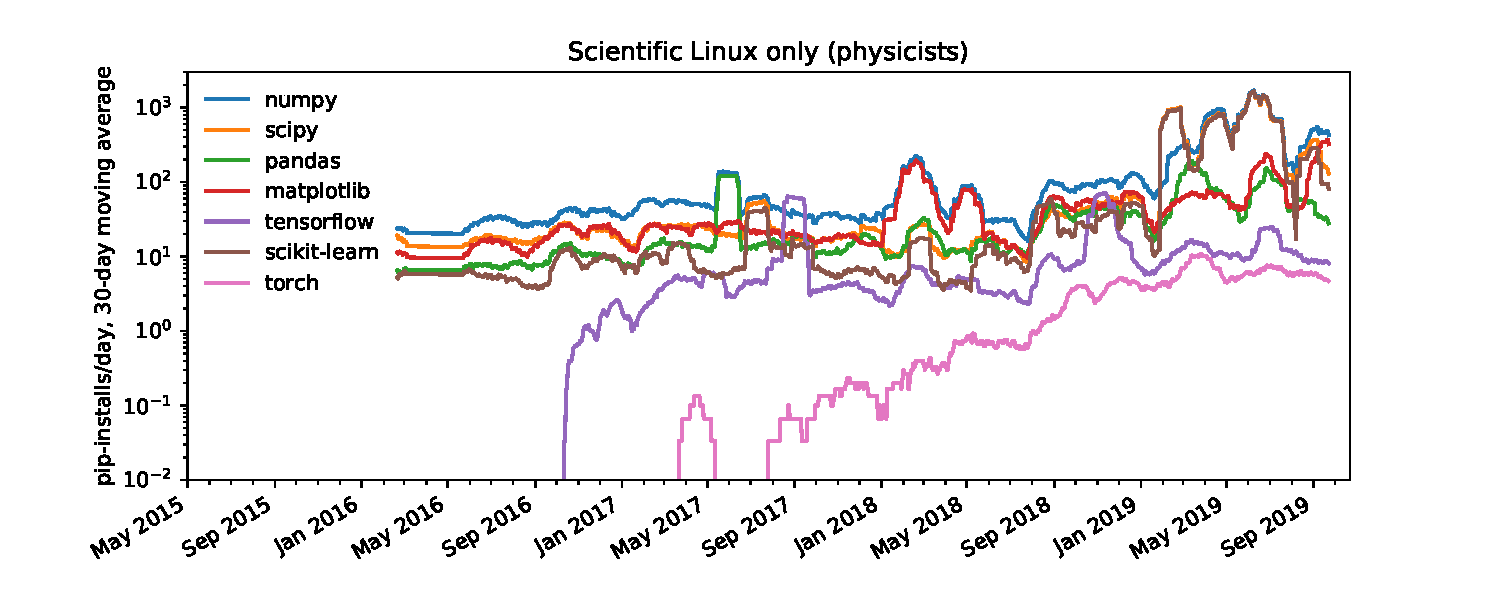
\includegraphics[width=\linewidth]{pip-scilinux-ml.pdf}
\end{columns}
\end{frame}

\begin{frame}{But take a step back and look in linear scale!}
\vspace{0.5 cm}
\begin{columns}
\column{1.2\linewidth}
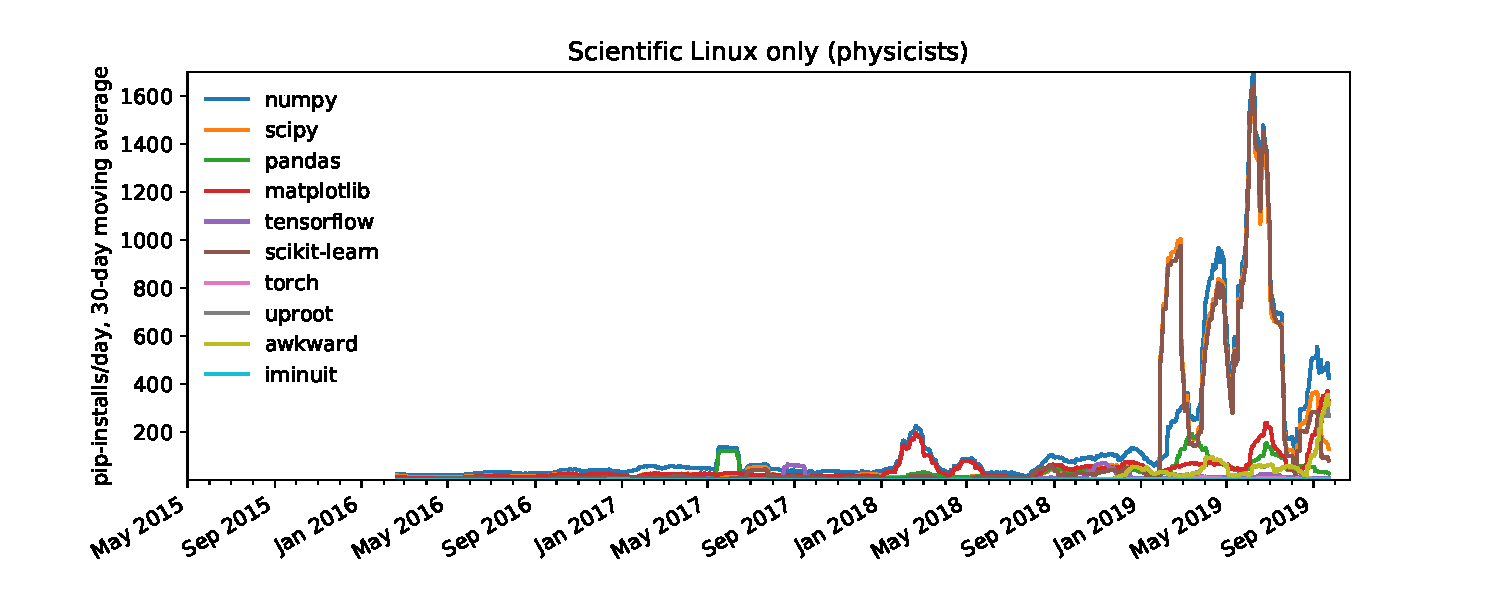
\includegraphics[width=\linewidth]{pip-scilinux-linear.pdf}
\end{columns}
\end{frame}

\begin{frame}{The bigger news is that more physicists are using Python {\it this year}}
\vspace{0.5 cm}
\begin{columns}
\column{1.2\linewidth}
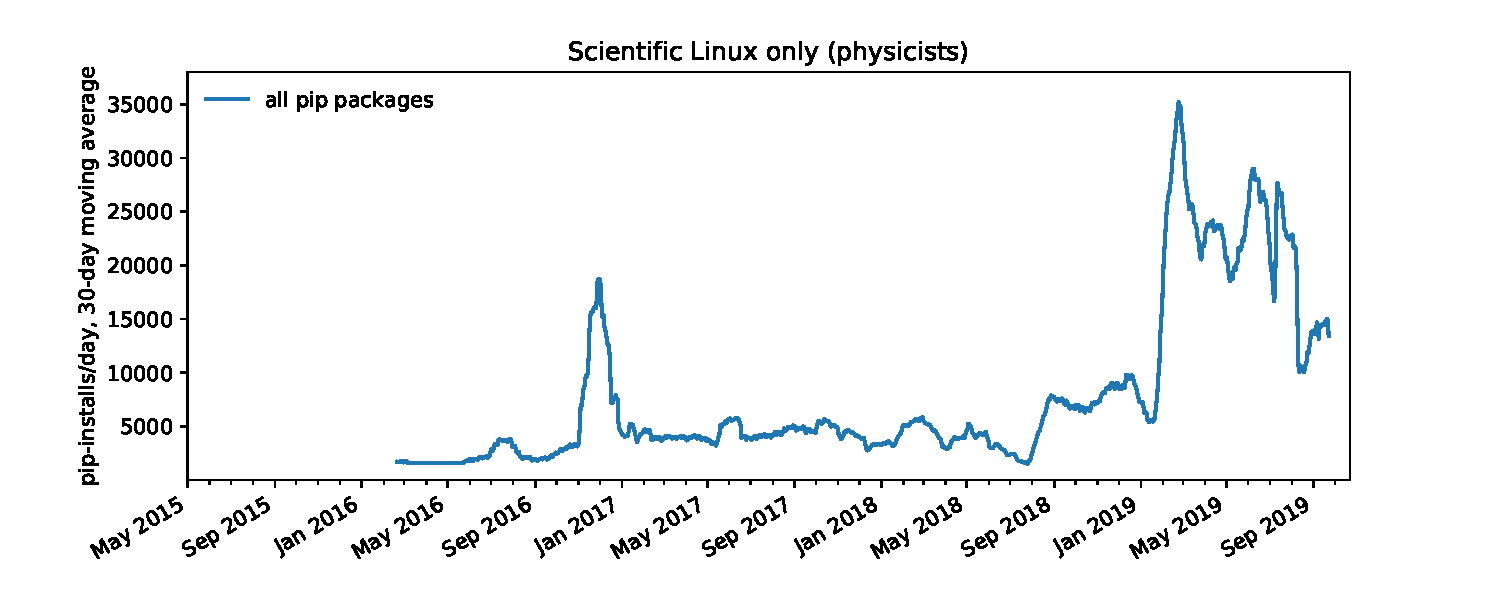
\includegraphics[width=\linewidth]{pip-scilinux-everything.pdf}
\end{columns}
\end{frame}

\begin{frame}{(In general, uproot is 4 orders of magnitude from Pandas)}
\vspace{0.5 cm}
\begin{columns}
\column{1.2\linewidth}
\only<1>{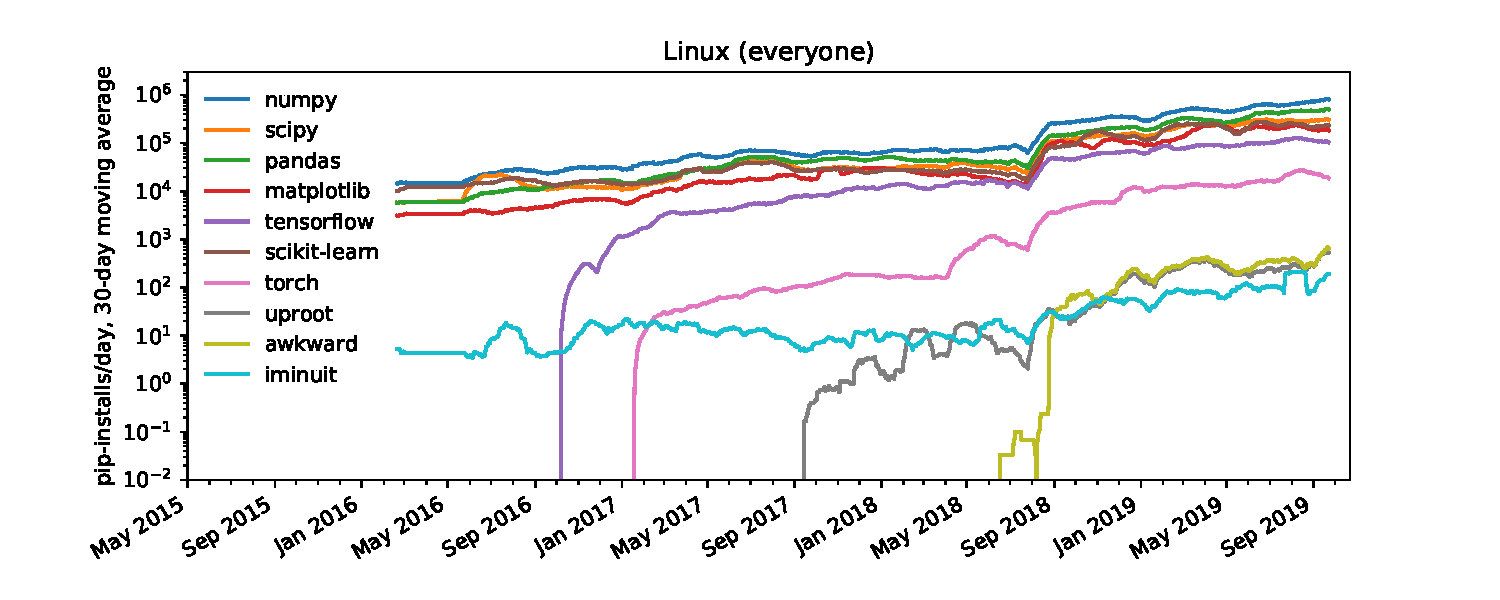
\includegraphics[width=\linewidth]{pip-linux.pdf}}\only<2>{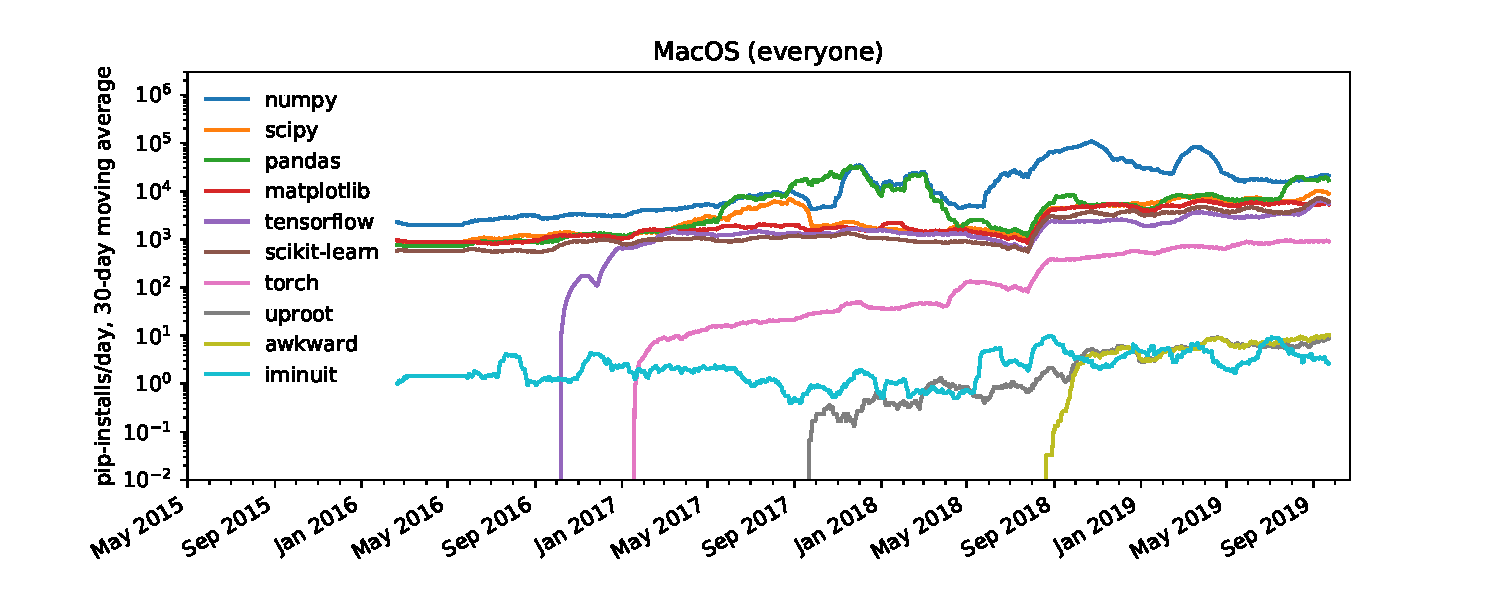
\includegraphics[width=\linewidth]{pip-macos.pdf}}\only<3>{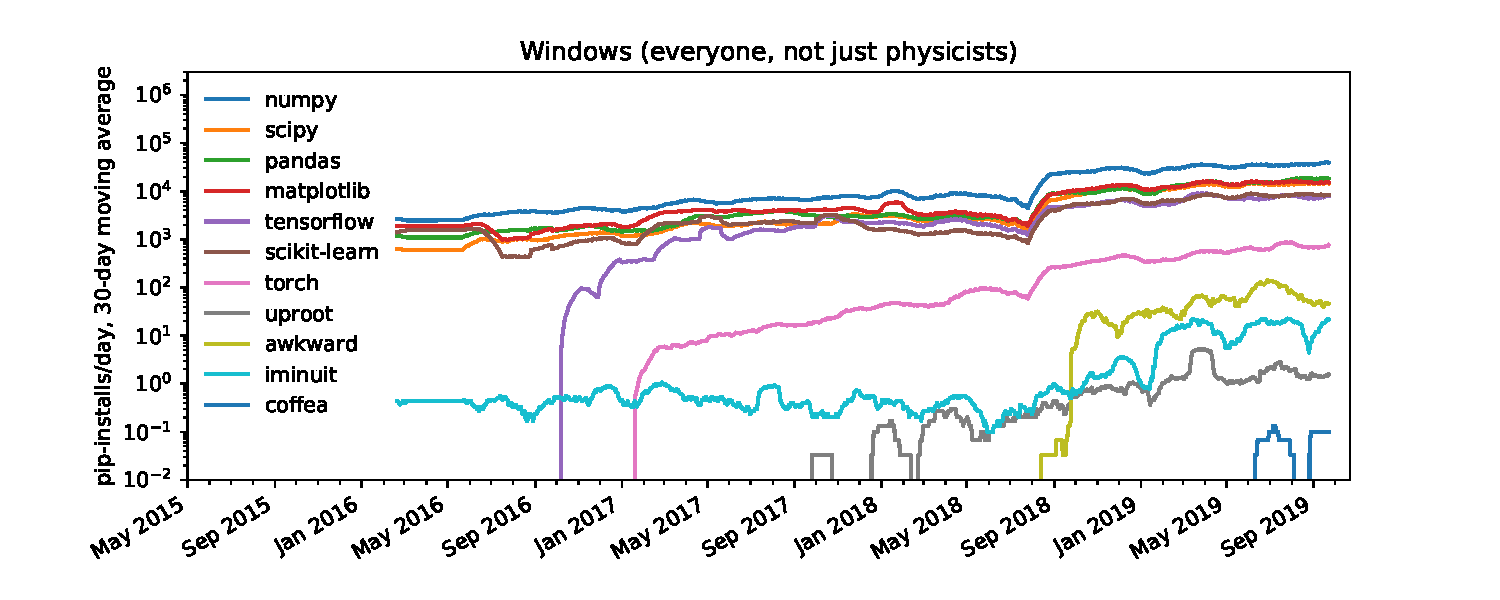
\includegraphics[width=\linewidth]{pip-windows.pdf}}
\end{columns}
\end{frame}

\begin{frame}{Another way to see Python usage among physicists: GitHub repos}
\begin{columns}
\column{1.2\linewidth}
\only<1>{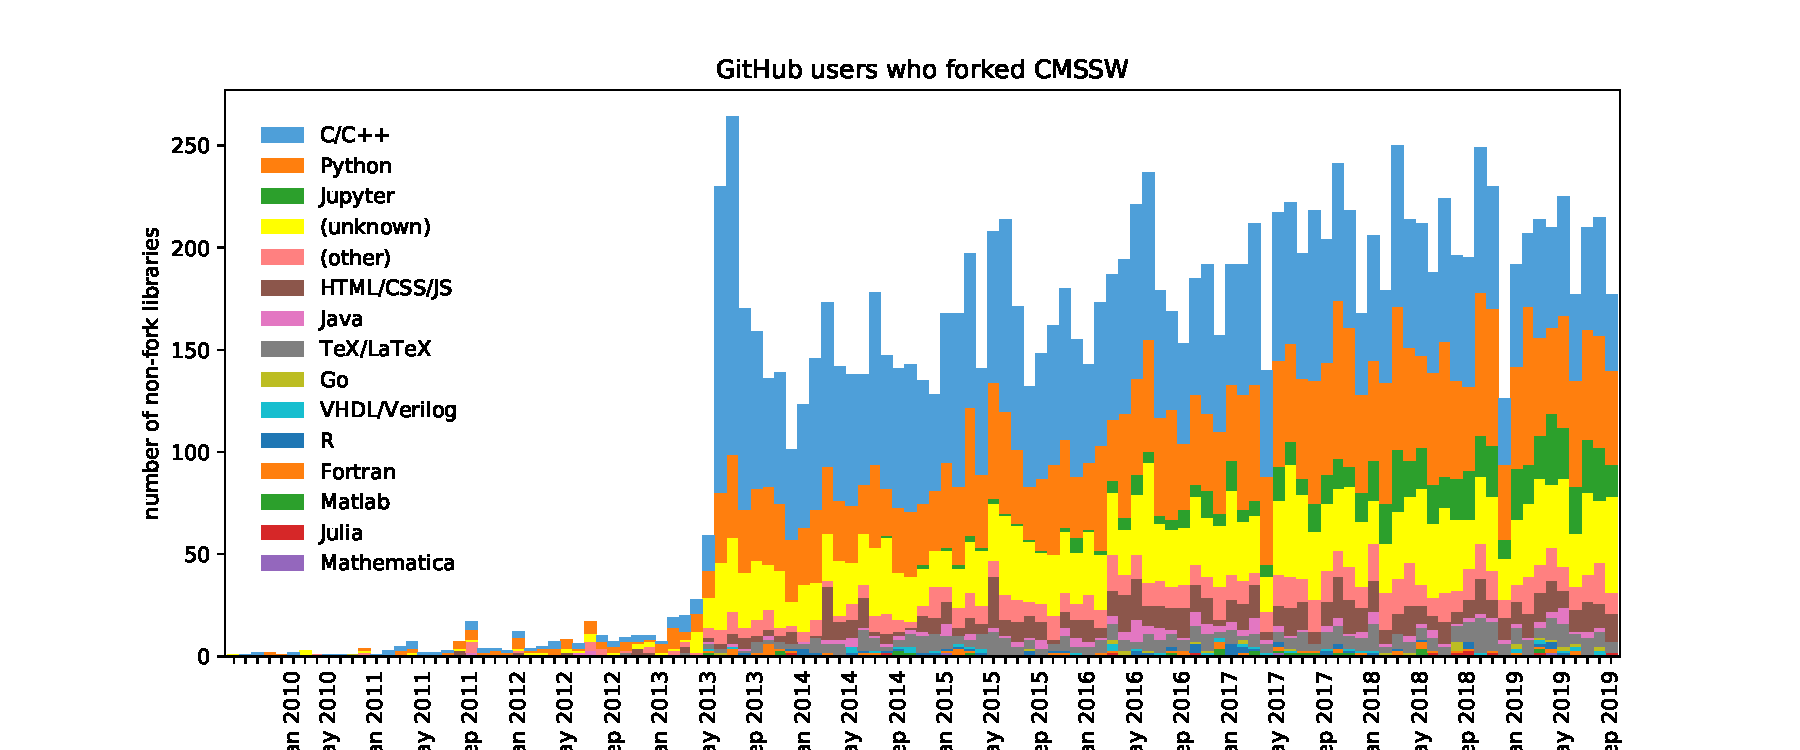
\includegraphics[width=\linewidth]{github-linear.pdf}}\only<2>{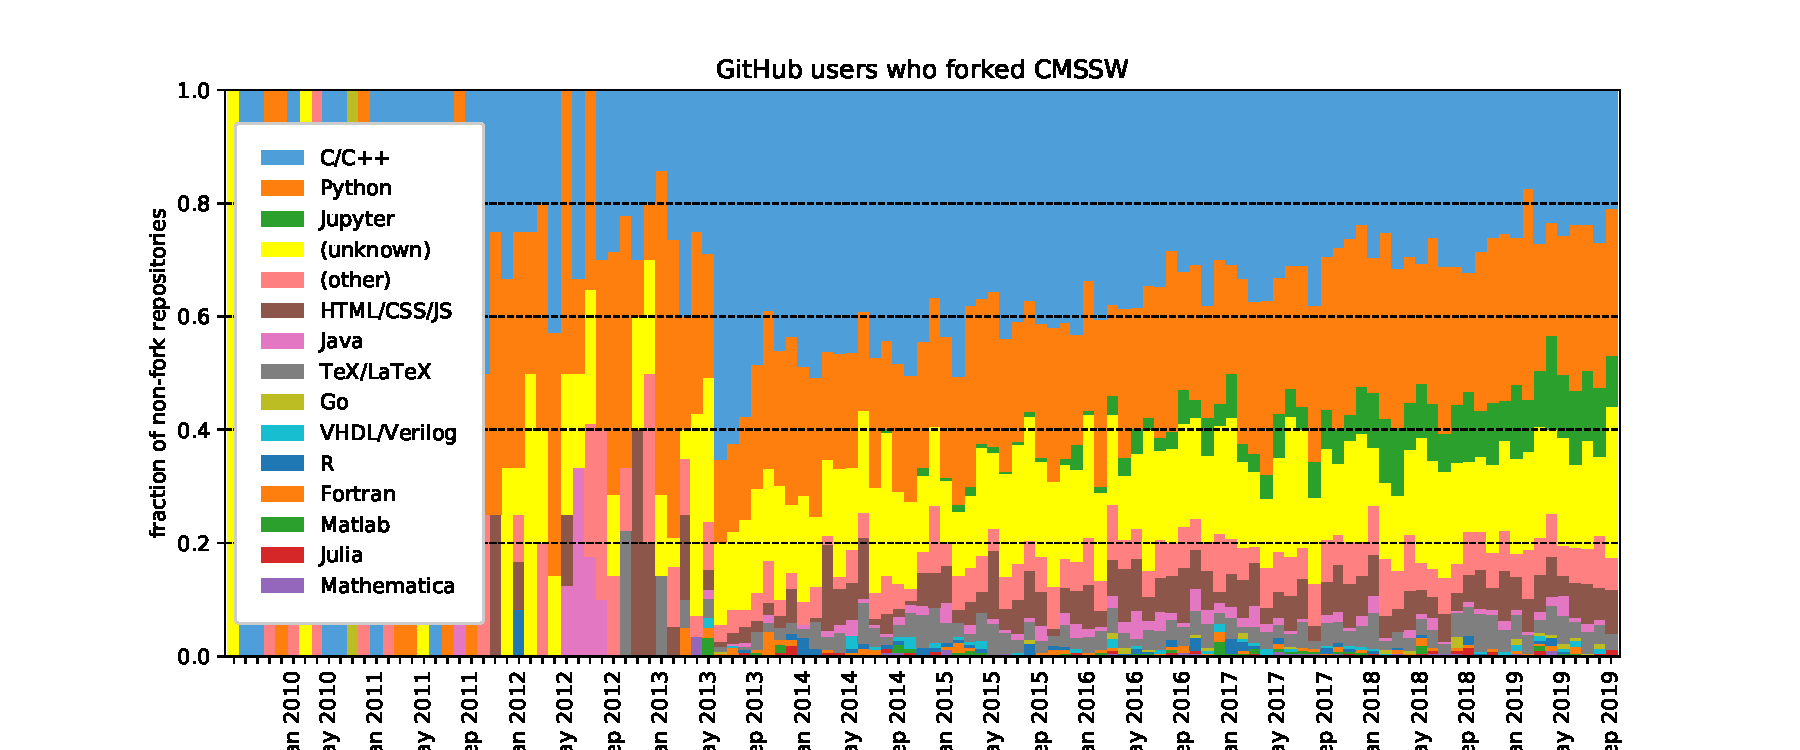
\includegraphics[width=\linewidth]{github-fraction.pdf}}\only<3>{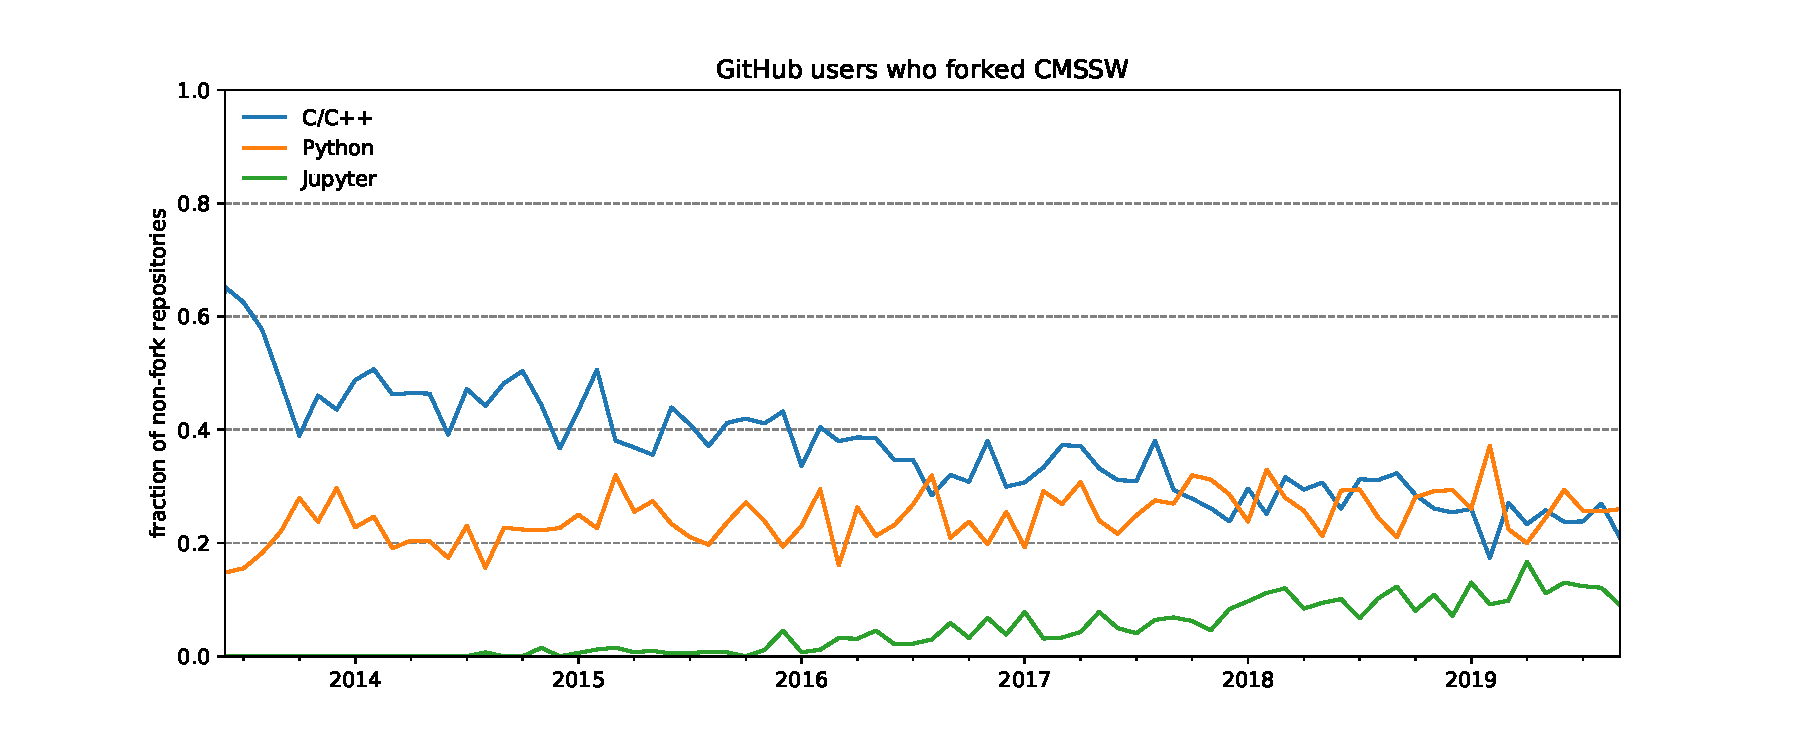
\includegraphics[width=\linewidth]{github-simplefraction.pdf}}
\end{columns}
\end{frame}

\begin{frame}{This is, in a sense, the third phase transition for our field}
\vspace{0.5 cm}
\begin{columns}
\column{1.1\linewidth}
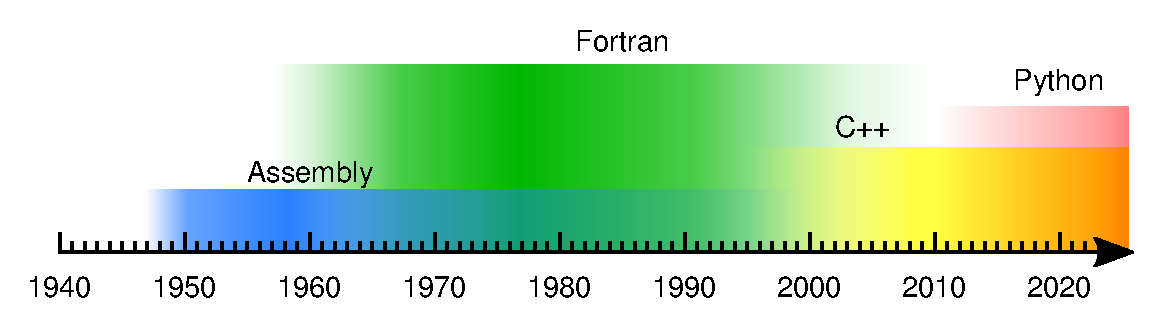
\includegraphics[width=\linewidth]{programming-languages.pdf}
\end{columns}
\end{frame}

\begin{frame}{Uproot/Awkward maintainance is pretty much constant}
\Large
\vspace{0.75 cm}
\begin{columns}
\column{0.36\linewidth}
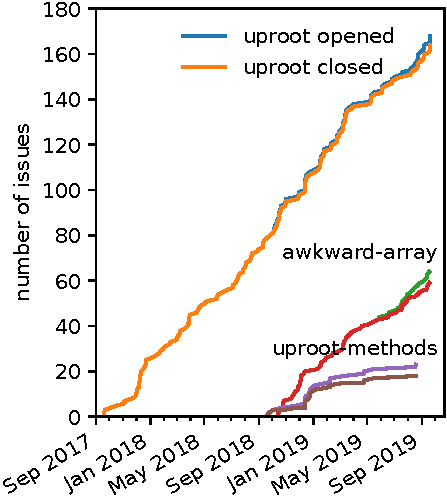
\includegraphics[width=\linewidth]{uproot-issues.pdf}

\column{0.72\linewidth}
\only<1>{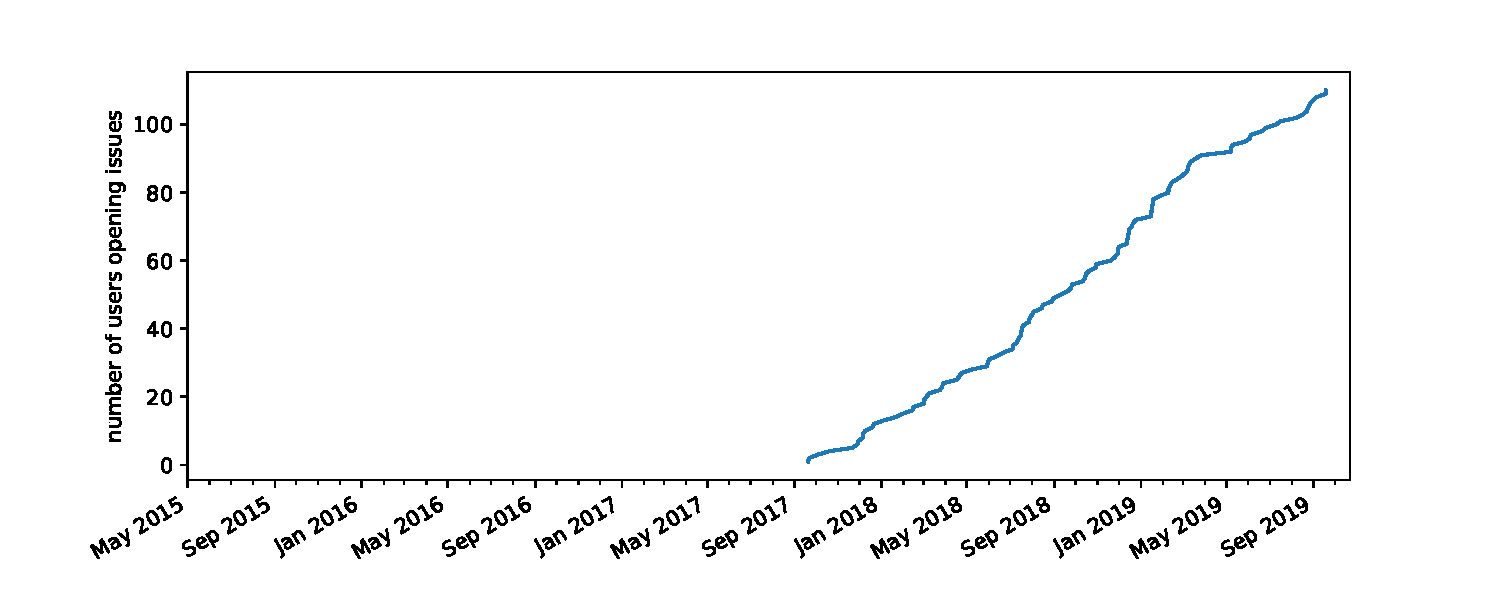
\includegraphics[width=0.5\linewidth]{uproot-users.pdf}\hfill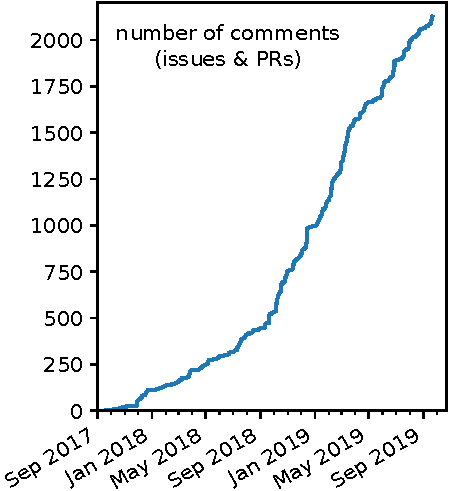
\includegraphics[width=0.5\linewidth]{uproot-comments.pdf}}\only<2->{\centering 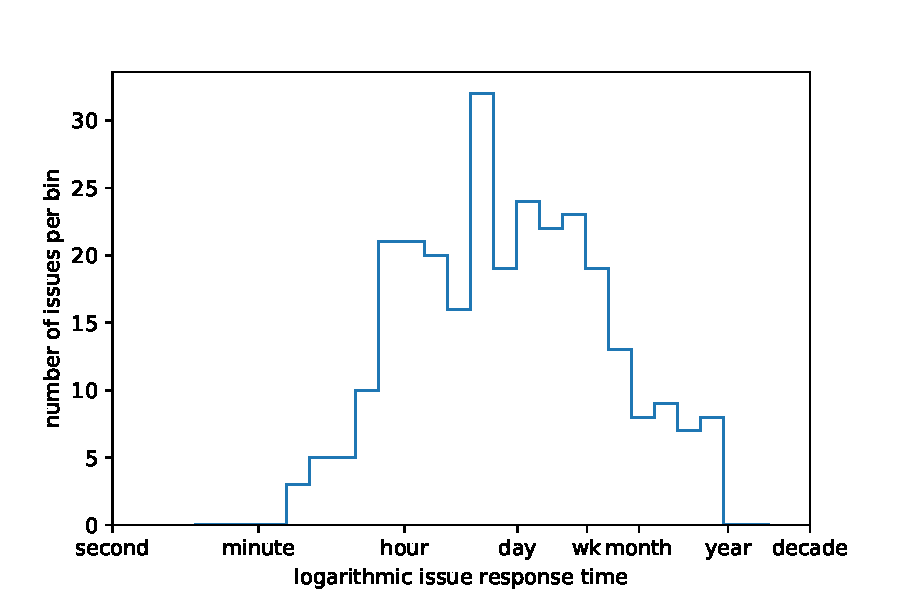
\includegraphics[width=0.45\linewidth]{uproot-response-time.pdf}}
\end{columns}

\vspace{0.25 cm}
\begin{center}
\uncover<3->{The problem with GitHub issues is that they go away, once closed.}
\end{center}
\end{frame}

\begin{frame}{Use StackOverflow!}
\begin{center}
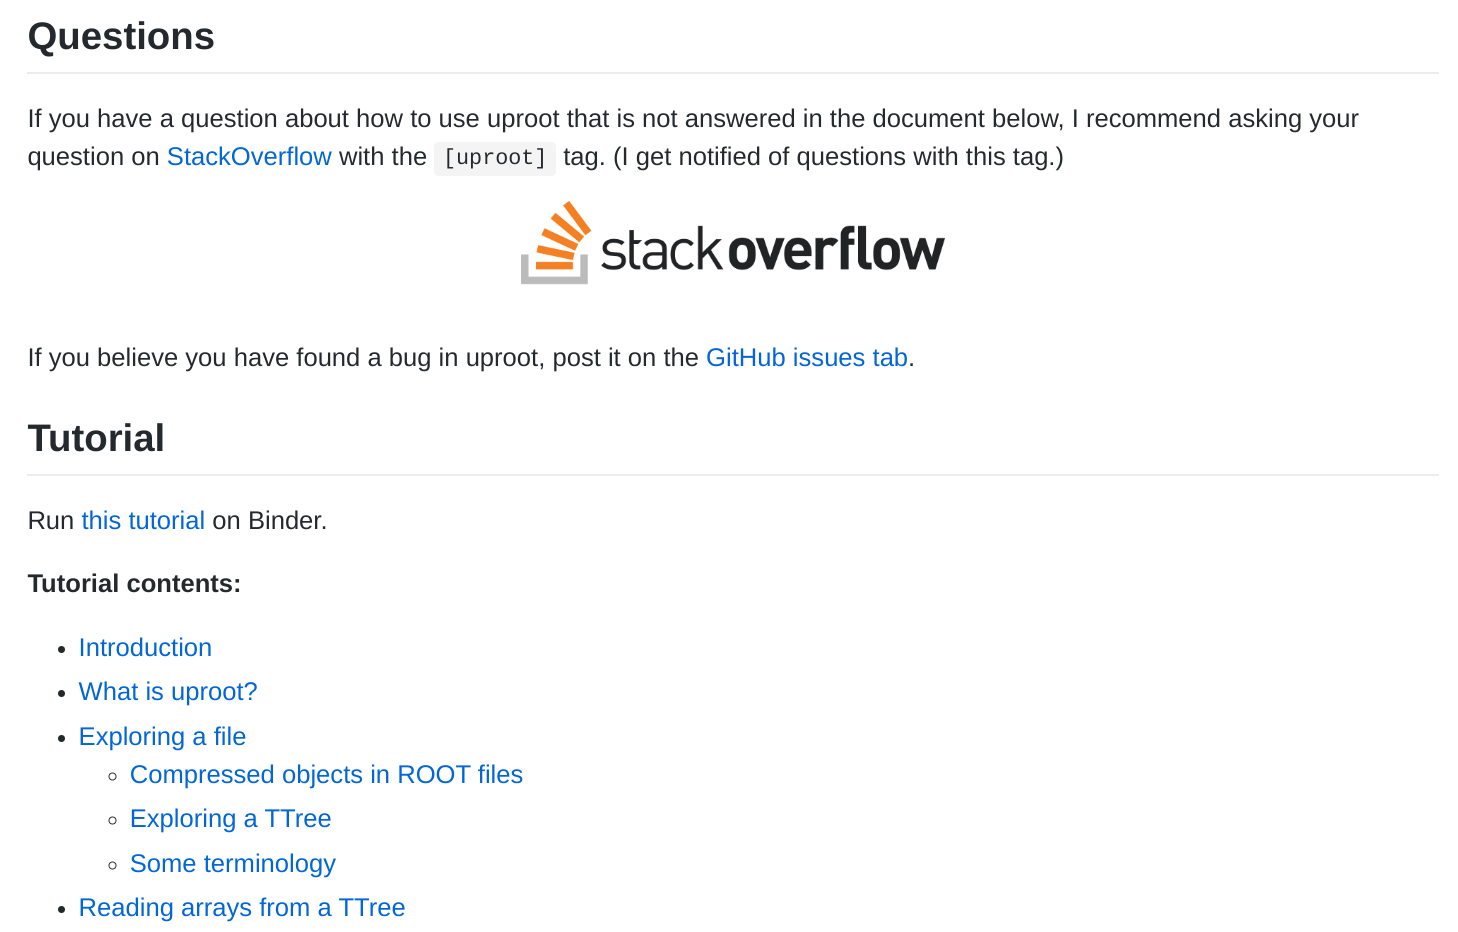
\includegraphics[width=0.88\linewidth]{uproot-stackoverflow.png}
\end{center}
\end{frame}

\begin{frame}{No, seriously, do it now.}
\vspace{0.15 cm}
\begin{columns}
\column{1.2\linewidth}
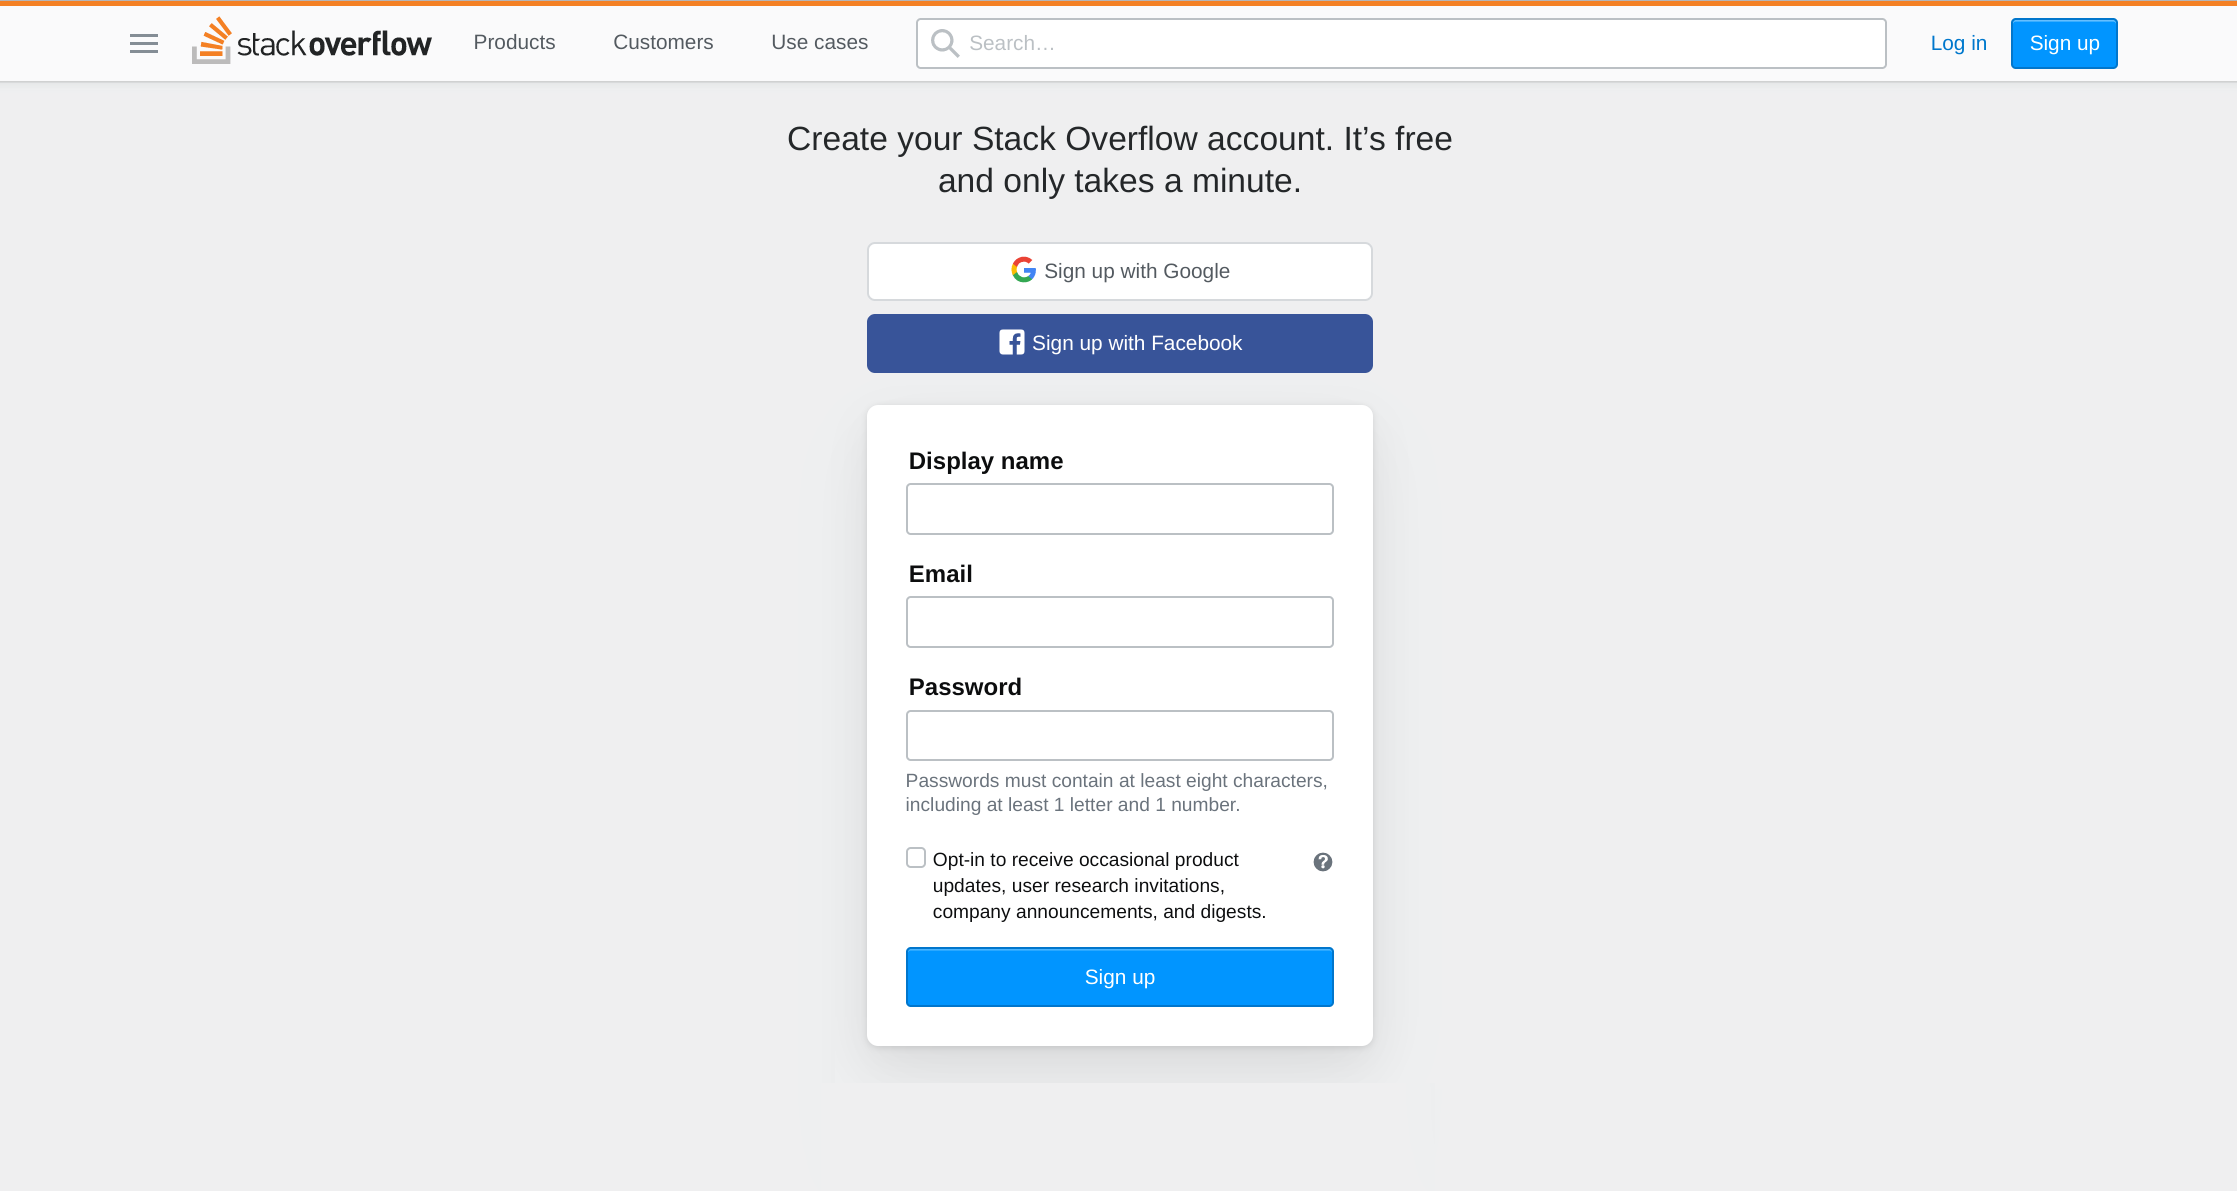
\includegraphics[width=\linewidth]{stackoverflow-signup.png}
\end{columns}
\end{frame}

\begin{frame}{}
\huge
\vspace{1 cm}
\begin{center}
\textcolor{darkblue}{Future of Uproot and Awkward}
\end{center}
\end{frame}

\begin{frame}{Future of uproot: maintenance}
\Large
\vspace{0.35 cm}
\begin{itemize}\setlength{\itemsep}{0.25 cm}
\item<1-> TTree-writing was the last {\it major} feature planned.
\item<2-> Bugs will be fixed.
\item<3-> Uproot will keep ahead of changes in ROOT I/O.

\vspace{0.05 cm}
\textcolor{gray}{\normalsize (Only one ROOT change has required intervention in uproot's two-year existence.)}

\item<4-> ROOT's future RNtuple can probably be handled with semi-independent code, as uproot-methods is now.
\item<5-> ``Uproot 4.0'' will be a transition to Awkward 1.0.
\end{itemize}

\normalsize
\vspace{0.25 cm}
\uncover<6->{\textcolor{gray}{(Apart from TTree-writing, uproot has been in maintenance mode for a year already.)}}
\end{frame}

\begin{frame}{Future of awkward: ``consolidation''}
\Large
\vspace{0.35 cm}
\begin{itemize}\setlength{\itemsep}{0.25 cm}
\item<1-> Awkward has been tested ``in the wild'' for a year now.
\item<2-> Pure Numpy implementation does some complex (clever!) things to perform jagged operations: no \mintinline{python}{for} loops allowed.

\vspace{0.1 cm}
\begin{itemize}\setlength{\itemsep}{0.2 cm}
\item<3-> \large There are limits to cleverness: many edge cases not handled.
\item<4-> \large Most frequent bugs are due to Numpy usage (e.g.\ \mintinline{python}{numpy.max([])}).
\item<5-> \large Desire to use awkward-arrays in Numba, on GPUs, and in C++ library interfaces leads to duplication; hard to synchronize implementations.
\end{itemize}

\item<6-> Feedback from users revealed some design mistakes.

\vspace{0.1 cm}
\begin{itemize}\setlength{\itemsep}{0.2 cm}
\item<7-> \large \mintinline{python}{a.cross(b)} versus \mintinline{python}{awkward.cross(a, b)}
\item<8-> \large User-visible \mintinline{python}{JaggedArray} versus \mintinline{python}{ChunkedArray(JaggedArray)}
\end{itemize}
\end{itemize}
\end{frame}

\begin{frame}{Rewrite/redesign in C and C++}
\large
\vspace{0.5 cm}
\begin{columns}
\column{0.5\linewidth}
\vspace{-0.2 cm}

\textcolor{darkblue}{Layer 1:} Python user interface.
\vspace{2\baselineskip}

\vspace{0.18 cm}
\textcolor{darkblue}{Layer 2:} Structure classes, ``layout''

(such as \mintinline{python}{JaggedArray}).
\vspace{\baselineskip}

\vspace{0.18 cm}
\textcolor{darkblue}{Layer 3:} Memory management, array allocation and ownership.
\vspace{2\baselineskip}

\vspace{0.18 cm}
\textcolor{darkblue}{Layer 4:} Implementations, where we write \mintinline{python}{for} loops. The only layer that needs to be optimized.

\column{0.5\linewidth}
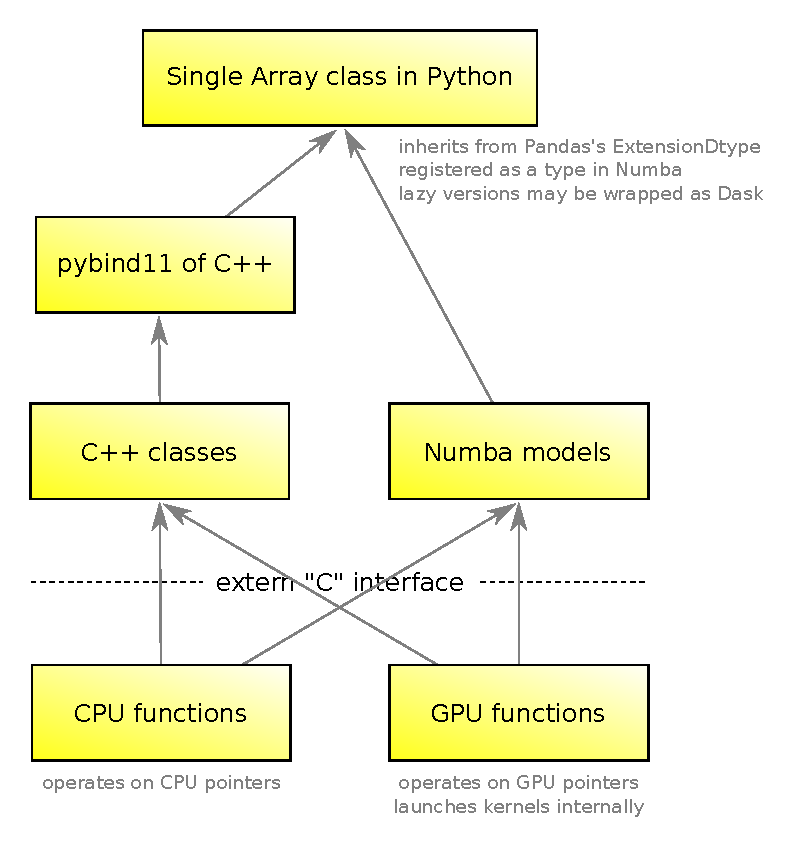
\includegraphics[width=\linewidth]{awkward-1-0-layers.pdf}
\end{columns}
\end{frame}



%% \begin{frame}{Not for lack of experience: I used C++ about as much as Python}
%% \vspace{0.5 cm}
%% \begin{columns}
%% \column{1.1\linewidth}
%% 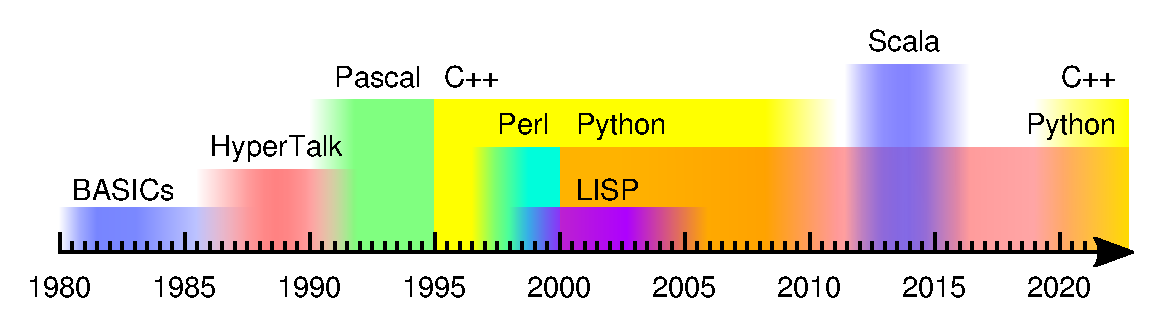
\includegraphics[width=\linewidth]{personal-programming-languages.pdf}
%% \end{columns}
%% \end{frame}

%% \begin{frame}{}
%% \huge
%% \vspace{1 cm}
%% \begin{center}
%% \textcolor{darkblue}{BACKUP}
%% \end{center}
%% \end{frame}

\end{document}
